\chapter{Contribuição: StarVZ sobre Spark} \label{ch:contribution}

A fase de pré-processamento do arcabouço StarVZ é similar a um fluxo de Ciência 
de Dados. Nele, são carregadas e manipuladas várias tabelas, utilizando 
bibliotecas do pacote \texttt{tidyverse}. Este Capítulo fala sobre as diferenças 
propostas e realizadas no StarVZ, com o objetivo de otimizar o tempo de 
execução da fase de pré-processamento. Resumidamente, no lugar de tabelas R, 
utilizaremos tabelas Spark (\emph{Spark Dataframes}) para o carregamento e manipulação de dados.
Na Seção \ref{sect:arch} são apresentadas as mudanças arquiteturais propostas
e na Seção \ref{sect:implement}, detalha-se a implementação dessas mudanças.

\section{Arquitetura Proposta} \label{sect:arch}

A arquitetura da aplicação que este trabalho se propõe a modificar pode ser 
visualizada na Figura \ref{fig:starvz-app}. Os dados, já em formato 
\textit{CSV} são lidos com a biblioteca \texttt{readr}. Com estes em memória, 
são realizadas filtragens e junções com o auxílio das bibliotecas \texttt{dplyr} 
e \texttt{tibble}. Finalmente, os dados são escritos em disco no formato 
\textit{Feather}, usando a biblioteca de mesmo nome. Todo esse processo é 
conduzido através de um código R.

\begin{figure}[ht]
 \centerline{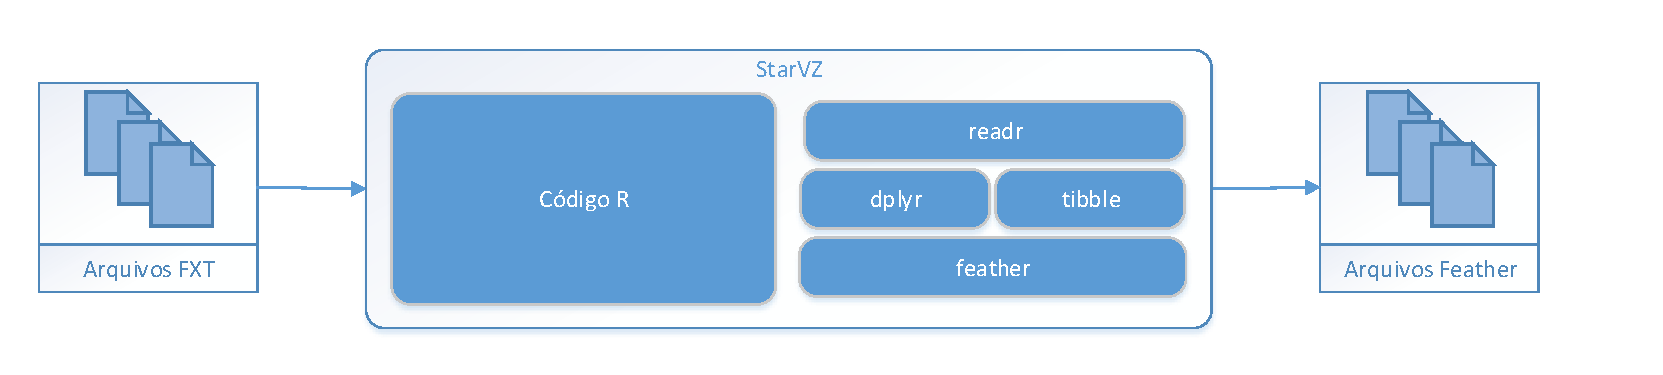
\includegraphics[width=1\textwidth]{./img/starvz-arch.pdf}}
 \caption{Arquitetura da aplicação StarVZ.}
 \label{fig:starvz-app}
\end{figure}

Durante o trabalho, identificou-se que não havia uma biblioteca que suportasse a 
escrita de tabelas Spark em arquivos \textit{Feather}. Isso é essencial para 
compararmos a escrita do mesmo tipo de dados tanto na execução sequencial quanto 
na distribuída. Devido ao ecossistema Hadoop utilizar 
o formato \textit{Parquet} \cite{ref:parquet} como padrão para armazenamento de 
dados colunares, a aplicação foi adaptada para escrever suas saídas neste 
formato. Isso foi realizado utilizando a biblioteca \texttt{Apache Arrow}, a 
arquitetura final da aplicação sequencial pode ser visualizada na Figura 
\ref{fig:starvz-app-arrow}. 

\begin{figure}[ht]
 \centerline{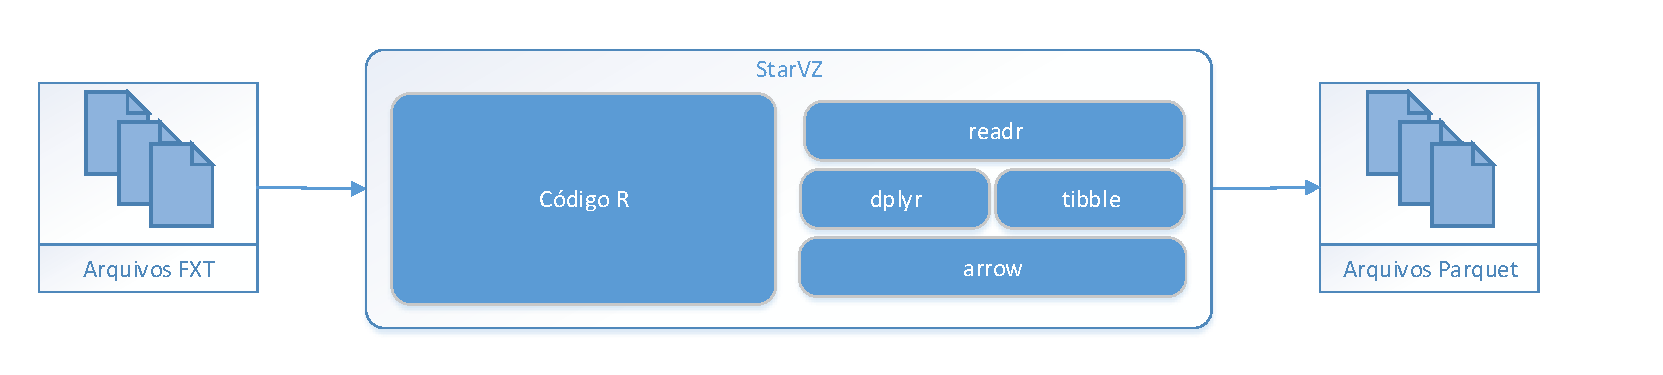
\includegraphics[width=1\textwidth]{./img/starvz-arch-arrow.pdf}}
 \caption{Arquitetura da aplicação StarVZ adaptada para escrever Parquet.}
 \label{fig:starvz-app-arrow}
\end{figure}

A Figura \ref{fig:starvz-app-spark} ilustra a arquitetura da aplicação após as 
modificações propostas. Considerando o tamanho dos arquivos de entrada, 
utilizaremos o HDFS para armazená-los. Todavia, alguns arquivos não crescem 
muito com o aumento do tamanho das entradas (seu tamanho fica na ordem de 
KBytes). Para estes, o custo de armazená-los e tratá-los no 
sistema de arquivos distribuído não é vantajoso pois os processamentos 
adicionais para realizar tais processos são mais caros que o tratamento do 
arquivo em si. Portanto, decidiu-se mantê-los com seu armazenamento e 
processamento sequencial.

\begin{figure}[ht]
 \centerline{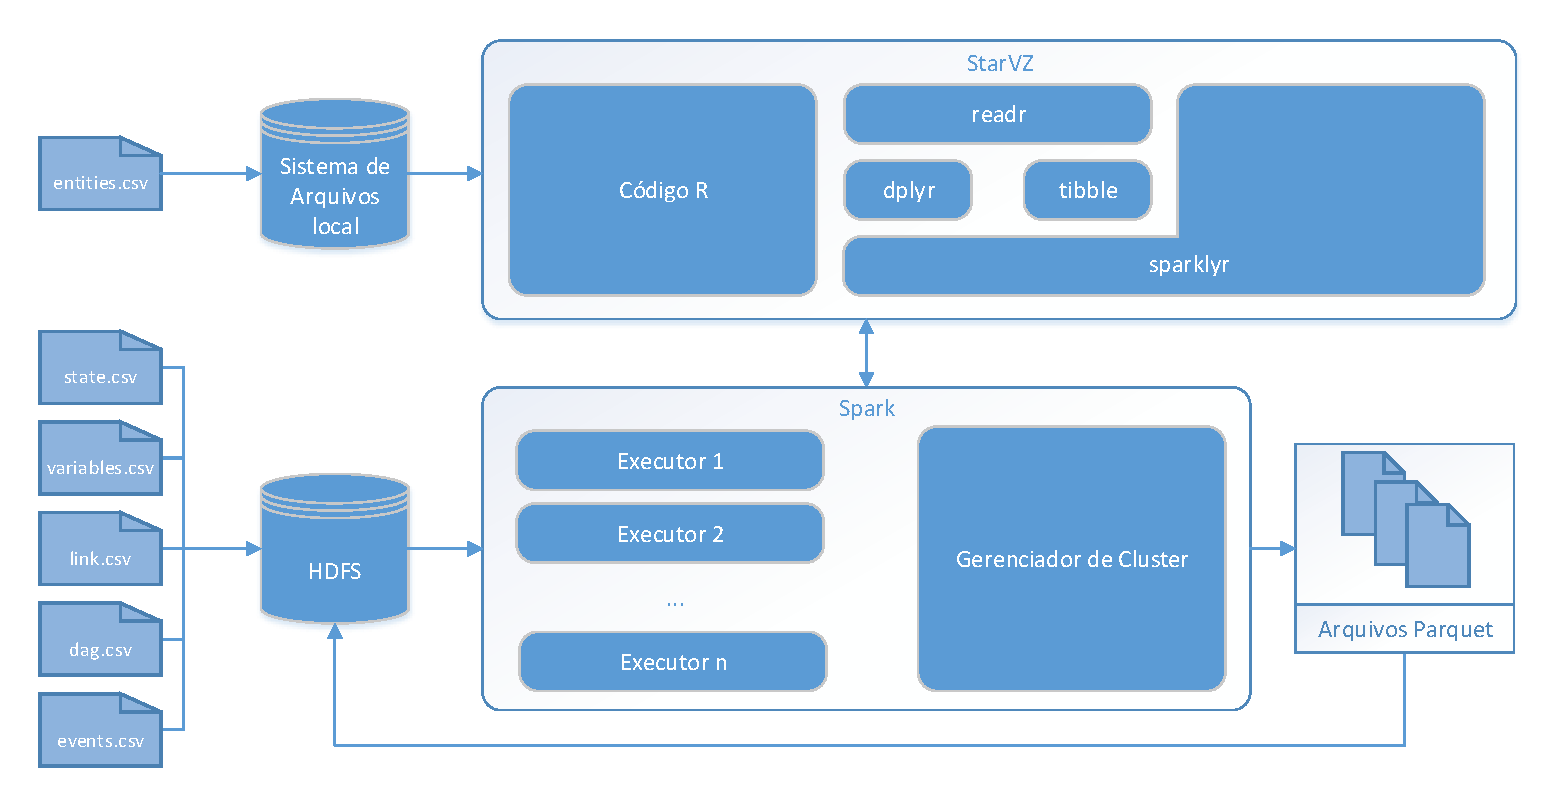
\includegraphics[width=1\textwidth]{./img/starvz-arch-spark.pdf}}
 \caption{Arquitetura da aplicação StarVZ utilizando Spark.}
 \label{fig:starvz-app-spark}
\end{figure}


A biblioteca escolhida para fazer a intermediação entre o código R e o Spark 
foi a \texttt{sparklyr}. De acordo com \citet{ref:sparkbook}, ela é 
baseada no pacote \texttt{dplyr} e sua abordagem prioriza a experiência com R, 
abstraindo alguns dos conceitos básicos como a seção Spark (\emph{Spark 
Session}), diferindo da abordagem padrão das APIs. O processo Driver é encapsulado
nas tratativas dessa biblioteca, que faz a intermediação entre o código R e a 
execução distribuída na infraestrutura. Devido a execução \emph{Lazy} da engine,
nem todas as operações realizadas em uma tabela geram tarefas distribuídas. Os
Executores utilizam diretamente o HDFS para leituras e escritas e mesmo aqueles
arquivos que foram mantidos com processamento sequencial são escritos no HDFS
para padronizar o local de saída.


\section{Implementação} \label{sect:implement}

Tratando-se dos detalhes de implementação, foi criado um novo arquivo com o 
fluxo de execução distribuída. Dessa forma, em um único pacote, o usuário pode 
optar por executar qualquer metodologia do arcabouço. Criou-se o parâmetro de 
tipo de execução, onde \texttt{-S} significa sequencial e \texttt{-D} significa 
distribuída, cada um com parâmetros específicos.

\begin{figure}[ht]
 \centerline{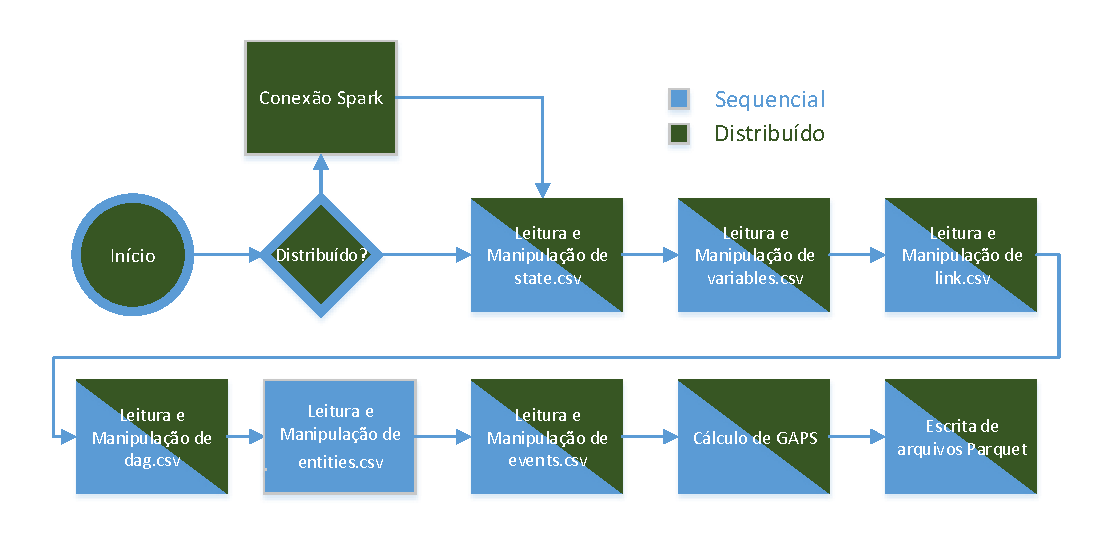
\includegraphics[width=1\textwidth]{./img/applicationflow.pdf}}
 \caption{Fluxo de execução da aplicação.}
 \label{fig:spark-starvz-flow}
\end{figure}

As modificações realizadas tiveram o objetivo de otimizar o processamento das 
tabelas. A ordem como elas são processadas não foi alterada, como pode ser 
visualizado na Figura \ref{fig:spark-starvz-flow}.

Na parte sequencial, a única modificação foi a escrita de arquivos no formato 
\textit{Parquet}, com o pacote \texttt{Apache Arrow}. Em termos de código, essa 
modificação é bastante pontual, adicionando uma importação de biblioteca e 
modificando os métodos de escrita de arquivos (de \texttt{write\_feather} 
para \texttt{write\_parquet}). É importante salientar que este pacote também 
conta com uma implementação de \texttt{write\_feather}, que é mais eficiente 
que aquela do pacote \texttt{feather}.

Para utilizar a \textit{Engine} e executar a aplicação de forma distribuída, é 
necessário estabelecer uma conexão Spark, utilizando o método 
\texttt{spark\_connect}. Com ela estabelecida, é possível ler arquivos em 
diversos formatos diretamente para tabelas no \texttt{sparklyr}. É importante 
ressaltar que com essa biblioteca, conseguimos ler arquivos armazenados no HDFS, 
o que permite que volumes de dados maiores que a quantidade de memória 
disponível na máquina sejam processados. Essa funcionalidade é muito importante 
pois desvincula o potencial da aplicação da limitação física da infraestrutura 
utilizada.

Com os arquivos carregados em tabelas Spark o restante do trabalho 
foi identificar equivalências entre as manipulações realizadas com \texttt{dplyr}
na \texttt{sparklyr}. Como esta foi desenvolvida baseada na primeira, esse 
processo foi facilitado. Ao encontrar uma manipulação, o seu resultado era 
observado na tabela original e reproduzido com funções suportadas pela 
\texttt{sparklyr}. Essa metodologia foi adotada pois, caso fosse necessário um 
tratamento que não fosse suportado pela biblioteca, seria preciso implementá-lo 
via funções definidas pelos usuários (\emph{User defined function ou UDFs}). 
Essa funcionalidade sofre de problemas de desempenho ao utilizar R ou Python 
pois há o custo de instanciar um processo R e compartilhar os dados de entradas 
e saídas. 

A Tabela \ref{tab:equivalence} exibe as principais equivalências de operações 
utilizadas em todas as tabelas. Enquanto a maior parte das operações possui uma 
equivalência de um pra um, a função \texttt{separate} necessita de um conjunto 
de manipulações para chegar no mesmo resultado. Ao aplicar essas equivalênias em 
todo o código, os dataframes foram validados um a um, comparando seu conteúdo. 

\begin{table}[H]
\centering
\begin{tabular}{l l} \toprule
\textbf{Operação \texttt{dplyr}}  &  \textbf{Operação \texttt{sparklyr}}\\ 
\midrule
distinct	& unique  \\
sort		& sdf\_sort \\
gsub		& regexp\_replace\\
rbind		& union\_all\\
grepl		& rlike\\
separate	& ft\_regex\_tokenizer + sdf\_separate\_column       \\
\end{tabular}
\caption{Equivalências de operações.}
\label{tab:equivalence}
\end{table}

A última manipulação de dados a ser realizada antes da escrita dos arquivos 
\textit{Parquet}, é um conjunto de funções recursivas. Durante o 
desenvolvimento, foi observada que a versão distribuída levava 
um tempo maior que a execução sequencial. Isso foi atribuído a avaliação \emph{Lazy} 
do Spark associado a recursividade, e foi um ponto de atenção 
levantado para ser observado durante os experimentos.

Por fim, as saídas são escritas no HDFS. Elas geram múltiplos arquivos, por 
exemplo, se a saída se chamar \emph{teste.parquet}, a aplicação criará uma pasta 
com esse nome e dentro dela haverá diversos arquivos, conforme abaixo. Isso 
ocorre pois por padrão as tabelas Spark são particionadas e escrevê-las gera um 
arquivo por partição.

\footnotesize
\begin{lstlisting}
 part-00000-1c143c87-5361-427c-825e-792497a8fa61-c000.snappy.parquet
 part-00001-1c143c87-5361-427c-825e-792497a8fa61-c000.snappy.parquet
 ...
\end{lstlisting}






